\chapter{Light Cones, Geodesics, and the Schwarzschild Horizon}

This lecture is constructed with some care. We do not begin with black holes, and we do not begin with Einstein's field equations. We begin by going back to special relativity and rebuilding the notions of time-like, space-like, and light-like intervals in the cleanest possible setting. Only then do we widen the metric to \(g_{\mu\nu}(x)\), turn geodesics into an action principle, check that the formalism reproduces Newton in the weak-field limit, and finally come to the Schwarzschild geometry and the horizon puzzle.

\section{Causal Structure in Minkowski Space}

For a small displacement in flat space-time, the proper-time element is
\begin{equation}
d\tau^2 = dt^2 - dx^2 - dy^2 - dz^2.
\end{equation}
Susskind briefly restores factors of \(c\), not for ornament but for bookkeeping:
\begin{equation}
d\tau^2 = dt^2 - \frac{dx^2+dy^2+dz^2}{c^2}.
\end{equation}
When we later take a nonrelativistic limit, those factors tell us what is small and what is not.

Now the crucial point is that \(d\tau^2\) is defined by this combination of differentials. It need not be positive just because the symbol looks like the square of something. Its sign depends on the balance between the time part and the space part. If
\begin{equation}
d\tau^2 > 0,
\end{equation}
the displacement is time-like: it has, so to speak, more time than space. If \(d\tau^2<0\), we define
\begin{equation}
ds^2 = -\,d\tau^2 = dx^2+dy^2+dz^2-dt^2,
\end{equation}
and then a space-like displacement is one for which \(ds^2>0\). The light-like case is the boundary between the two:
\begin{equation}
d\tau^2 = 0
\qquad\Longleftrightarrow\qquad
dt^2 = dx^2+dy^2+dz^2
\quad (c=1).
\end{equation}

This classification is organized by the light cone. The surface of the cone is the light-like set, its interior is the time-like region, and its exterior is the space-like region. The lecture insists on a small geometric point that is worth keeping: the cone is the shell, not the filled interior. Light rays lie on the cone itself.

\begin{figure}[t]
\centering

\includegraphics[width=0.78\textwidth]{lecture_05_figure_02.png}
\caption{Light cone and space-like interval in Minkowski space. The board groups the proper-time element, the space-like interval, and the causal diagram into a single classification picture.}
\end{figure}

\begin{figure}[t]
\centering
\begin{tikzpicture}[scale=1.0]
\draw[->] (0,-2.3) -- (0,2.3);
\draw[->] (-2.4,0) -- (2.4,0);
\draw (-1.6,1.6) -- (0,0) -- (1.6,1.6);
\draw (-1.6,-1.6) -- (0,0) -- (1.6,-1.6);
\fill (0,0) circle (1.4pt);
\draw[->,thick] (0,0) -- (0,1.2);
\draw[->,thick] (0,0) -- (0,-1.2);
\draw[->,thick] (0,0) -- (1.6,0.35);
\end{tikzpicture}
\caption{A clean redraw of the causal classification used in the lecture. Time-like directions lie inside the cone, space-like directions outside it, and light-like directions on the cone itself.}
\end{figure}

Proper time is not a formal convenience. Along a time-like trajectory it is the time that a clock on the trajectory actually reads. Likewise, in the space-like case the quantity \(s\) is proper distance, the distance measured by meter sticks. These are already physical notions in special relativity, and the lecture wants them firmly in hand before curvature enters.

\section{Signature, Metrics, and Local Light Cones}

The flat metric may be written in matrix form as
\begin{equation}
\eta_{\mu\nu}=\mathrm{diag}(-1,1,1,1).
\end{equation}
Here one should speak carefully. The metric is a rank-two tensor, not literally ``that matrix'' in every coordinate system. The matrix is its expression in a particularly simple coordinate frame. In the sign convention of this lecture,
\begin{equation}
d\tau^2 = -\,g_{\mu\nu}\,dx^\mu dx^\nu,
\end{equation}
so that \(g_{\mu\nu}dx^\mu dx^\nu\) is positive on space-like displacements.

At this point the lecture makes a conceptual correction. The invariant content is not that there is one preferred arrow on the board that deserves to be called time. The invariant content is that the metric has one negative eigenvalue and three positive ones. That is the Lorentzian signature:
\begin{equation}
\mathrm{signature}(g_{\mu\nu}) = (-,+,+,+).
\end{equation}
A world with two negative eigenvalues would be a world with two time directions, and Susskind simply refuses to entertain it as physics.

Now we widen the scope. In curved space-time the metric is not \(\eta_{\mu\nu}\), but
\begin{equation}
g_{\mu\nu}=g_{\mu\nu}(x).
\end{equation}
At every event \(x\), there is a matrix \(g_{\mu\nu}(x)\), and at every event that matrix must still have one negative and three positive eigenvalues. This means that at every point there is a light cone. Its appearance may change from point to point; it may look tipped, tilted, or squashed. But the causal story remains the same: inside the cone time-like, outside space-like, on the cone light-like.

\begin{figure}[t]
\centering

\includegraphics[width=0.82\textwidth]{lecture_05_figure_03.png}
\caption{Position-dependent metric and local light-cone sketches. The left board still carries the time-like, space-like, and light-like classification, while the right board introduces \(g_{\mu\nu}(x)\) and the idea of a cone at each point.}
\end{figure}

\begin{figure}[t]
\centering
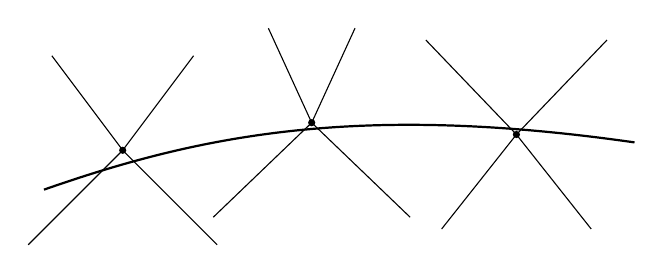
\begin{tikzpicture}[scale=1.0]
\draw[thick] (-4,-0.5) .. controls (-2,0.2) and (0,0.6) .. (3.5,0.1);
\foreach \x/\y/\a/\b in {-3/0/0.9/1.2, -0.6/0.35/0.55/1.25, 2.0/0.2/1.15/0.95} {
  \fill (\x,\y) circle (1.3pt);
  \draw (\x,\y) -- ++(-\a,1.2);
  \draw (\x,\y) -- ++(\a,1.2);
  \draw (\x,\y) -- ++(-\b,-1.2);
  \draw (\x,\y) -- ++(\b,-1.2);
}
\end{tikzpicture}
\caption{A cleaned companion drawing of neighboring local light cones. Their apparent shape changes with coordinates and with the local metric, but the causal classification does not.}
\end{figure}

What changes, then, when the cone seems to change shape? Often nothing but coordinates. One may squash a cone by rescaling the spatial axes, or tilt it by using more awkward coordinates, without changing the underlying geometry at all. The lecture returns to this point several times because it is exactly the sort of confusion that will come back later at the Schwarzschild horizon.

\subsection{Question \& Answer}

A natural question is this: if there is one negative eigenvalue, does that pick out one unique time-like vector?

No. The invariant statement is about the form, not about a unique physical arrow. In a diagonal coordinate system one may indeed point to the vector \((1,0,0,0)\), but that is a coordinate-basis statement. It is not the real content of the metric. All time-like vectors inside the cone are related to one another by Lorentz transformations. The point is not that the metric has chosen one preferred vector; the point is that the metric has Lorentzian signature.

This is why one must be careful not to identify the shape drawn on the board with the invariant content. The board may display one axis as ``time,'' but the true statement is more abstract and more stable: one negative direction, three positive ones, and therefore a causal cone at each event.

\section{Geodesics from Stationary Distance to Stationary Proper Time}

The lecture now changes gears. Up to this point we have been fixing the causal vocabulary. The next step is to say how particles move. Susskind briefly recalls the earlier, more differential definition of a geodesic. In standard notation, with dots now denoting derivatives with respect to proper time,
\begin{equation}
\ddot x^\mu + \Gamma^\mu{}_{\sigma\rho}\dot x^\sigma\dot x^\rho = 0.
\end{equation}
The spoken discussion around the sign of the Christoffel term is hesitant, so it is better to write the standard clean form and move on.

For actual calculation, the lecture prefers a different definition. In ordinary space, a geodesic is the curve of stationary distance between two points. If the spatial metric is \(g_{mn}\), then
\begin{equation}
ds^2 = g_{mn}\,dx^m dx^n,
\qquad
\int ds = \int \sqrt{g_{mn}\,dx^m dx^n}.
\end{equation}
The geodesic is the curve that makes this integral stationary.

Now comes the deliberate transition. We are no longer interested in ordinary distance on a surface. We are interested in proper time in space-time. So we write
\begin{equation}
\tau = \int \sqrt{-\,g_{\mu\nu}\,dx^\mu dx^\nu},
\end{equation}
and for a massive particle we define the action
\begin{equation}
A = -m\tau = -m\int \sqrt{-\,g_{\mu\nu}\,dx^\mu dx^\nu}.
\end{equation}
This is the point at which geometry becomes mechanics.

In the live lecture the proper-time functional is repeatedly described as something to minimize. The clean statement is slightly subtler. A time-like geodesic makes the proper time stationary and, locally, maximal. Because the action has the extra minus sign, the same curve minimizes \(A=-m\tau\). The sign is not decoration; it is exactly what makes the variational problem look like the familiar principle of least action.

\section{Particle Action, Lagrangian Form, and Euler--Lagrange Equations}

At first sight the proper-time action looks strange. It does not look like an ordinary integral over a single variable with a recognizable integrand. This is why Susskind pauses here in the lecture and spends time on the rewrite. We divide the quadratic form inside the square root by \(dt^2\) and compensate by pulling one factor of \(dt\) outside:
\begin{align}
A
&= -m\int \sqrt{-\,g_{\mu\nu}(x)\,dx^\mu dx^\nu} \\
&= -m\int \sqrt{-\,g_{\mu\nu}(x)\,\frac{dx^\mu}{dt}\frac{dx^\nu}{dt}}\,dt.
\end{align}
Here the time component contributes \(dt/dt=1\), while the spatial components contribute ordinary velocities.

Now the action has the conventional form
\begin{equation}
A=\int L\,dt,
\end{equation}
with
\begin{equation}
L=-m\sqrt{-\,g_{\mu\nu}(x)\,\dot x^\mu\dot x^\nu},
\qquad
\dot x^\mu \equiv \frac{dx^\mu}{dt}.
\end{equation}
This is the real payoff of the rewrite. The square-root worldline functional is no longer exotic. It is simply a Lagrangian, a function of positions and velocities, exactly of the kind to which Euler--Lagrange applies.

\begin{figure}[t]
\centering

\includegraphics[width=0.82\textwidth]{lecture_05_figure_05.png}
\caption{Relativistic particle action rewritten as an integral of the Lagrangian. The board preserves the live transition from the square-root worldline functional to the conventional action form \(A=\int L\,dt\).}
\end{figure}

\begin{figure}[t]
\centering

\includegraphics[width=0.82\textwidth]{lecture_05_figure_06.png}
\caption{The same action a little later, with the Lagrangian isolated more cleanly.}
\end{figure}

There is also a small sign question in the lecture at this point: is the quantity under the square root actually positive? Yes. For a genuine massive particle the trajectory is time-like, so \(-g_{\mu\nu}\dot x^\mu\dot x^\nu>0\). Real particles do not travel on space-like worldlines.

\subsection{Question \& Answer}

Why does the expression under the square root count as the Lagrangian?

Because once the action has been rewritten in the conventional form \(A=\int L\,dt\), the integrand is, by definition, the Lagrangian. But there is more to it than a mere label. The entire point of the rewrite is that minimizing the action is now equivalent to applying the Euler--Lagrange equations to this specific function of positions and velocities.

Thus we recover the familiar machinery of mechanics:
\begin{equation}
\frac{d}{dt}\left(\frac{\partial L}{\partial \dot x^\mu}\right)=\frac{\partial L}{\partial x^\mu}.
\end{equation}
This is exactly the move the lecture wants to make: from ``here is an action'' to ``here is a differential equation.'' In that sense the geodesic equation becomes a force-like law, the relativistic analogue of an \(F=ma\)-type equation.

\section{Weak-Field Metric and the Newtonian Limit}

Now the lecture comes to the first real physical application. We want a metric for the gravitational field of a spherically symmetric object, but before trusting any guess we must check that it reproduces Newton when the field is weak and the motion is slow.

We begin from flat space-time,
\begin{equation}
d\tau^2 = dt^2 - \frac{1}{c^2}(dx^2+dy^2+dz^2),
\end{equation}
and we alter only the \(dt^2\) coefficient at first:
\begin{equation}
d\tau^2 = \left(1+\frac{2u(x)}{c^2}\right)dt^2 - \frac{1}{c^2}(dx^2+dy^2+dz^2).
\end{equation}
The new function \(u(x)\) is the Newtonian gravitational potential. The lecture's point is explicit: let us check that this ansatz really gives Newton's equation when particles move slowly.

Substituting this metric into the worldline action, and restoring the factor of \(c^2\) demanded by dimensions, we obtain
\begin{equation}
A=-mc^2\int \sqrt{1+\frac{2u(x)}{c^2}-\frac{\dot{\mathbf x}^{\,2}}{c^2}}\,dt,
\qquad
\dot{\mathbf x}^{\,2}=\dot x^2+\dot y^2+\dot z^2.
\end{equation}
At this stage the lecture makes an important practical remark. If we simply threw away every \(1/c^2\) term, we would throw away the entire effect. The right thing to do is to expand the square root around \(1\):
\begin{equation}
\sqrt{1+\epsilon}\simeq 1+\frac{\epsilon}{2},
\qquad
\epsilon=\frac{2u-\dot{\mathbf x}^{\,2}}{c^2}.
\end{equation}
Therefore
\begin{align}
L
&= -mc^2\sqrt{1+\frac{2u-\dot{\mathbf x}^{\,2}}{c^2}} \\
&\simeq -mc^2\left(1+\frac{2u-\dot{\mathbf x}^{\,2}}{2c^2}\right) \\
&\simeq -mc^2 - m\,u(x) + \frac{m}{2}\dot{\mathbf x}^{\,2}.
\end{align}
The constant term \(-mc^2\) is irrelevant. A constant in the Lagrangian disappears when we differentiate. What remains is exactly the nonrelativistic Lagrangian \(T-U\):
\begin{equation}
L_{\mathrm{nr}} = \frac{m}{2}\dot{\mathbf x}^{\,2} - m\,u(x).
\end{equation}
Applying the Euler--Lagrange equations yields
\begin{equation}
m\ddot{\mathbf x} = -m\nabla u.
\end{equation}

This is the checkpoint the lecture needs before proceeding. The geometric action does indeed reduce to ordinary mechanics in the appropriate limit. In particular, we learn that to first order in \(1/c^2\),
\begin{equation}
g_{00}\approx 1+\frac{2u}{c^2}.
\end{equation}
For a source of mass \(M\),
\begin{equation}
u(r)=-\frac{GM}{r},
\end{equation}
so the time-time part of the metric becomes
\begin{equation}
g_{00}\approx 1-\frac{2GM}{rc^2}.
\end{equation}
This is not yet the full Schwarzschild metric, but it is the bridge from Newtonian intuition to the relativistic answer.

\section{Schwarzschild Metric and the Horizon Puzzle}

Only now do we turn to the main target: the metric outside a static, spherically symmetric gravitating body. Since this is a central-force problem, the lecture naturally switches to spherical coordinates. In the convention used on the board, \(\theta\) is measured from the equator rather than from the north pole, so
\begin{equation}
d\Omega^2 = d\theta^2 + \cos^2\theta\,d\phi^2,
\end{equation}
and flat three-space becomes
\begin{equation}
dx^2+dy^2+dz^2 = dr^2 + r^2 d\Omega^2.
\end{equation}
That is why we are doing polar coordinates here: not because they are prettier, but because they are the natural coordinates for the motion around a central mass.

Using the weak-field result, the first guess is
\begin{equation}
d\tau^2 \approx \left(1-\frac{2GM}{rc^2}\right)dt^2
- \frac{1}{c^2}\left(dr^2+r^2d\Omega^2\right).
\end{equation}
If we define the Schwarzschild radius
\begin{equation}
r_s = \frac{2GM}{c^2},
\end{equation}
this becomes
\begin{equation}
d\tau^2 \approx \left(1-\frac{r_s}{r}\right)dt^2
- \frac{1}{c^2}\left(dr^2+r^2d\Omega^2\right).
\end{equation}
The lecture writes this down, pauses, and then says bluntly that something is terribly wrong with it.

The problem is one of signature. Far from the source, all is well. But when \(r<r_s\), the coefficient of \(dt^2\) becomes negative. If the spatial terms are left untouched, then every diagonal term has the same sign. We would have lost the Lorentzian signature altogether. In effect, we would have wandered into a region with no time-like direction at all.

\subsection{Question \& Answer}

Why must the coefficient of \(dr^2\) change when the coefficient of \(dt^2\) changes sign?

Because the metric must remain Lorentzian. If the \(dt^2\) coefficient flips sign, one of the other coefficients must flip with it. By spherical symmetry the radial term is the natural candidate. The angular sphere remains what it is; it is the radial piece that can exchange roles with the time piece.

Einstein's equations give the precise correction:
\begin{equation}
d\tau^2
=
\left(1-\frac{r_s}{r}\right)dt^2
-
\frac{1}{c^2\left(1-\frac{r_s}{r}\right)}dr^2
-
\frac{r^2}{c^2}d\Omega^2.
\end{equation}
This is the Schwarzschild metric in the form used in the lecture. When \(r\) passes below \(r_s\), both the \(dt^2\) and \(dr^2\) coefficients change sign. The signature remains Lorentzian. In these coordinates the role of \(t\) and \(r\) flips: \(t\) becomes space-like and \(r\) becomes time-like.

That sounds mysterious, and the lecture does not try to hide the mystery. But it immediately adds the crucial warning: this is a feature of Schwarzschild coordinates, not yet evidence that something locally disastrous happens at the horizon. In fact the lecture insists that the geometry is perfectly smooth there; it is the coordinates that have become awkward.

To see how motion works, we first set \(c=1\). For purely radial infall the angular variables do not change, so \(d\Omega=0\), and the metric reduces to
\begin{equation}
d\tau^2
=
\left(1-\frac{r_s}{r}\right)dt^2
-
\frac{1}{1-\frac{r_s}{r}}\,dr^2.
\end{equation}
Now divide through by \(dt^2\) and multiply by \(dt\). The action becomes ordinary again, and the radial Lagrangian is
\begin{equation}
L=-m\sqrt{\left(1-\frac{r_s}{r}\right)-\frac{\dot r^2}{1-\frac{r_s}{r}}},
\qquad
\dot r \equiv \frac{dr}{dt}.
\end{equation}
The lecture then uses the fact that energy is conserved. Let us set
\begin{equation}
a(r)=1-\frac{r_s}{r}.
\end{equation}
Then
\begin{equation}
L=-m\sqrt{a-\frac{\dot r^2}{a}}.
\end{equation}
The conjugate momentum is
\begin{equation}
p_r=\frac{\partial L}{\partial \dot r}
=
\frac{m\dot r}{a\sqrt{a-\dot r^2/a}},
\end{equation}
and the Hamiltonian is
\begin{equation}
H=p_r\dot r-L
=
\frac{ma}{\sqrt{a-\dot r^2/a}}.
\end{equation}
Since \(L\) has no explicit \(t\)-dependence, \(H\) is conserved. Writing \(H=E\) and solving for \(\dot r\) gives
\begin{equation}
\dot r^2
=
a^2\left(1-\frac{m^2}{E^2}a\right)
=
\left(1-\frac{r_s}{r}\right)^2
\left[1-\frac{m^2}{E^2}\left(1-\frac{r_s}{r}\right)\right].
\end{equation}
The live algebra in the lecture becomes garbled here, but the clean reconstruction is straightforward. Its main consequence is the one the lecture emphasizes: near the horizon the bracket tends to \(1\), so
\begin{equation}
\dot r \sim \pm\left(1-\frac{r_s}{r}\right)
\qquad
(r\to r_s).
\end{equation}
Thus the infalling particle, described in Schwarzschild coordinate time \(t\), slows down and asymptotically freezes at the horizon.

The lecture then says there is a much easier way to see the same effect. Forget the massive particle for a moment and look at a radial light ray. A light ray satisfies
\begin{equation}
d\tau^2=0.
\end{equation}
So in the radial Schwarzschild metric,
\begin{equation}
\left(1-\frac{r_s}{r}\right)dt^2
-
\frac{1}{1-\frac{r_s}{r}}\,dr^2
=0.
\end{equation}
Multiplying by \(1-r_s/r\) gives
\begin{equation}
\left(1-\frac{r_s}{r}\right)^2dt^2 = dr^2,
\end{equation}
and therefore
\begin{equation}
\frac{dr}{dt}=\pm\left(1-\frac{r_s}{r}\right).
\end{equation}
The two signs correspond to outgoing and ingoing rays. In either case, as \(r\to r_s\),
\begin{equation}
\frac{dr}{dt}\to 0.
\end{equation}
Even light appears to get stuck in these coordinates.

\subsection{Question \& Answer}

Why does the horizon take infinite Schwarzschild time to reach but only finite proper time to cross?

Because the two times are not the same clock. The outside observer uses Schwarzschild coordinate time \(t\). The infalling observer uses proper time \(\tau\). Near the horizon,
\begin{equation}
\frac{dr}{dt}\sim -\left(1-\frac{r_s}{r}\right),
\end{equation}
so
\begin{equation}
\frac{dt}{dr}\sim -\,\frac{1}{1-r_s/r}
=
-\,\frac{r}{r-r_s}.
\end{equation}
This has a logarithmic divergence at \(r=r_s\). So the coordinate time needed to reach the horizon is infinite.

But that does not mean the infalling observer waits forever. The coefficient multiplying \(dt^2\) in the metric goes to zero at the horizon, so a large coordinate interval \(dt\) can correspond to a small proper interval \(d\tau\). This is exactly the physical content of the late discussion in the lecture about clocks near the horizon: a given amount of outside time corresponds to a smaller and smaller proper time in the falling car. Hence the infalling observer reaches the horizon in finite proper time even while the outside observer says the crossing is never completed.

The same distinction resolves the apparent contradiction about the speed of light. A photon has Schwarzschild coordinate speed \(dr/dt\to 0\), but that is not its local speed in a freely falling frame. Locally the photon still travels at the speed of light. The horizon does not turn photons into massive particles, and it does not make clocks stop. The pathology is in the Schwarzschild coordinates, not in the local physics.

This is also why the lecture insists that there is nothing geometrically singular at the horizon. The light cones are perfectly healthy there; one simply needs better coordinates to see that fact transparently. Radar tracking from outside becomes misleading because the reflected signal takes longer and longer to return and is redshifted more and more severely. The outside observer therefore describes the infalling object as flattening, slowing, and piling up near the horizon, while the infalling observer simply sails through.

One further caution is essential. The Schwarzschild solution is an exterior solution. For the Earth, the Schwarzschild radius is about a centimeter, far inside the real matter distribution. There is no Earth horizon. The Schwarzschild metric is the correct vacuum geometry outside the source. Only when the entire body collapses within its Schwarzschild radius does the horizon become physically relevant.

The lecture closes by leaving one last knot tied rather than untied. If nothing ever seems to cross the horizon in outside time, how can a black hole grow? Susskind says explicitly that the conclusion ``therefore a black hole can never grow'' sounds right but is wrong. The resolution is postponed. That is the right place to stop: with the geometry established, the coordinate artifact identified, and the deeper global question still alive.

\section{Summary}

The lecture unfolds in a deliberately staged way. We begin in Minkowski space so that time-like, space-like, and light-like intervals are concrete before curvature enters. We then shift from the picture of a single drawn cone to the invariant statement about Lorentzian signature, and from there to a general metric \(g_{\mu\nu}(x)\) with a local light cone at each event.

Next comes the methodological turn. Instead of treating geodesics only through Christoffel symbols, we turn the problem into a variational one. The proper-time functional becomes a particle action, the action becomes a Lagrangian, and Euler--Lagrange turns geometry into equations of motion. In the weak-field limit that machinery reproduces Newton and shows that \(g_{00}\approx 1+2u/c^2\) to first order.

Only then do we arrive at the Schwarzschild metric. The first guess, which modifies only the time component, fails because it destroys the Lorentzian signature near the Schwarzschild radius. The corrected metric preserves the signature, but in Schwarzschild coordinates it makes both infalling particles and light rays appear to freeze at the horizon. The lecture's real lesson is that this freezing is a coordinate effect. Proper time remains finite, local physics remains regular, and the horizon is not a place where the geometry breaks. It is a place where the argument, having become truly interesting, is ready to continue.